\chapter{Automi a pila}

Un PDA è un automa che ha lo stesso potere computazionale delle CFG.
Solo i PDA non deterministici definiscono tutti i CFL.

Ma la versione deterministica è il modello per i parser. 

La maggior parte dei linguaggi di programmazione ha PDA deterministici.

\subsubsection{Intuizione}

Bisogna pensare a un NFA con il potere aggiuntivo di poter manipolare una pila (o stack).
Le sue azioni sono determinate da:
\begin{enumerate}
    \item Lo stato in cui si trova (del suo "NFA"),
    \item Il simbolo input letto (o $\epsilon$), e
    \item Il simbolo letto sul top della sua pila.
\end{enumerate}
Essendo non deterministico, un PDA può scegliere l'azione successiva in un insieme di possibili scelte.

Per ciascuna scelta, il PDA può:
\begin{enumerate}
    \item Cambiare stato, e anche
    \item Cambiare il simbolo sul top della pila con una sequenza di zero o più simboli.
    \begin{itemize}
        \item Zero simboli = "pop."
        \item Più simboli = sequenza di "push."
    \end{itemize}
\end{enumerate}

\subsubsection{Definizione formale di PDA}
Un PDA è descritto da:
\begin{itemize}
    \item Un insieme finito di stati (Q, generalmente).
    \item Un alfabeto di simboli input ( $\Sigma$, generalmente).
    \item Un alfabeto di simboli di stack ( $\Gamma$, generalmente).
    \item Una funzione di transizione ( $\delta$, generalmente).
    \item  Uno stato iniziale $\left(\mathrm{q}_{0}\right.$, in $\mathrm{Q}$, generalmente $)$.
    \item Un simbolo iniziale $\left(Z_{0}\right.$, in $\Gamma$, generalmente).
    \item Un insieme di stati finali $(F \subseteq Q$, in genere).
\end{itemize}

\subsubsection{Convenzioni}
\begin{itemize}
    \item $a, b, \ldots$ sono simboli di input. (Ma a volte permettiamo che $\epsilon$ sia un possibile valore).
    \item $\ldots$, X, Y, Z sono simboli di pila.
    \item $\ldots, w, x, y, z$ sono stringhe di simboli input.
    \item $\alpha, \beta, \ldots$ sono stringhe di simboli di pila.
\end{itemize}

\subsubsection{La funzione di transizione}
Dipende da tre argomenti:
\begin{enumerate}
    \item Uno stato, in Q.
    \item  Un input, che è $o$ un simbolo in $\Sigma$ o $\epsilon$.
    \item Un simbolo di stack in $\Gamma$.
\end{enumerate}
$\delta(q, a, z)$ è un insieme di zero o più coppie della forma $(p, \alpha)$.

p è uno stato; $\alpha$ è una stringa di simboli di pila.

\subsubsection{Azioni del PDA}
Se $\delta(q, a, Z)$ contiene $(p, \alpha)$ tra le sue possibili coppie, allora quello che il PDA può fare nello stato $\mathrm{q}$, con input a $\mathrm{e}$ con $Z$ sul top dello stack è:
\begin{enumerate}
    \item  Cambiare stato, passando da q a p.
    \item "Cancellare" a dall'input (ma a potrebbe essere $\epsilon$ ).
    \item Rimpiazzare Z sul top dello stack con $\alpha$.
\end{enumerate}

\subsubsection{Esempio: PDA}
Definire un PDA che accetti

$\quad\left\{0^{n} 1^{n} \mid n \geq 1\right\}$.

Gli stati:
\begin{itemize}
    \item $q=$ a stato iniziale. Siamo nello stato q se
abbiamo visto solo 0 .
    \item $p=$ abbiamo visto almeno un 1 e ora
possiamo procedere solo se i simboli input
sono 1.
    \item $f=$ stato finale; accettazione (se ha letto
tutto l'input).
\end{itemize}
I simboli dello stack:
\begin{itemize}
    \item $Z_{0}=$ simbolo iniziale. Indica anche il fondo della pila, così sappiamo quando avremo contato lo stesso numero di 1 e di $0 .$
    \item $X=$ marcatore, usato per contare il numero di 0 visti nell'input.
\end{itemize}
Le transizioni:
\begin{itemize}
    \item $ \delta\left(q, 0, Z_{0}\right)=\left\{\left(q, X Z_{0}\right)\right\} .$
    \item $ \delta(q, 0, X)=\{(q, X X)\} .$ Queste due regole
permettono l'inserimento di una $X$ nella pila per
ogni 0 letto dall'input.
    \item $ \delta(q, 1, X)=\{(p, \epsilon)\} .$ Quando vede un 1, il
PDA va nello stato p ed elimina una $X .$
    \item $ \delta(p, 1, X)=\{(p, \epsilon)\} .$ Elimina una $X$ per ogni $1 .$
    \item $ \delta\left(p, \epsilon, Z_{0}\right)=\left\{\left(f, Z_{0}\right)\right\} .$ Accetta se vede il fondo
$($ e ha letto tutto l'input).
\end{itemize}

\subsubsection{Azioni del PDA dell'esempio}

\begin{figure}[hbpt!]
    \centering
    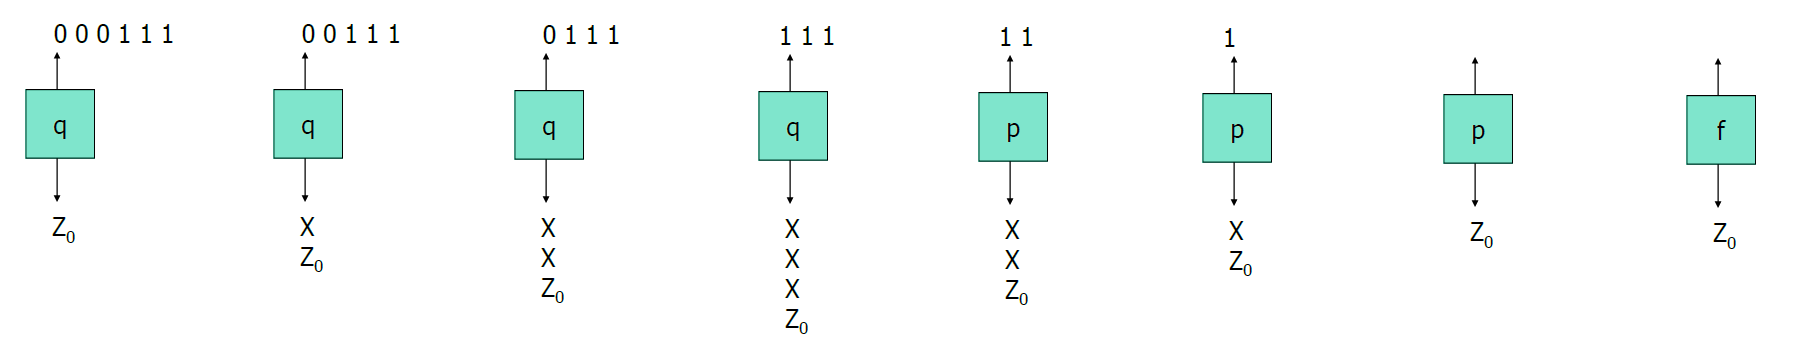
\includegraphics[width=\textwidth]{./Images/6.1.png}
\end{figure}
\FloatBarrier


\subsubsection{Descrizioni istantanee}
Possiamo formalizzare le figure viste con una descrizione istantanea (ID).
Una ID è una tripla $(q, w, \alpha)$, dove:
\begin{enumerate}
    \item q è lo stato (corrente).
    \item w è l'input residuo.
    \item $\alpha$ è il contenuto dello stack, sommità a sinistra (top $\rightarrow$ down corrisponde a left $\rightarrow$ right).
\end{enumerate}

\subsubsection{Trasformazioni di ID}

Per dire che la ID I può diventare la ID J in un'azione del PDA, scriveremo $I \vdash J$. Formalmente, $(q, a w, X \alpha) \vdash(p, w, \beta \alpha)$ per ogni we $\alpha$, se $\delta(q, a, X)$ contiene $(p, \beta)$. Estendiamo $+$ a $\vdash^{*}$, per rappresentare "zero o più mosse":
\begin{itemize}
    \item Base: I $\vdash^{*}$ I.
    \item Induzione: Se $I \vdash^{*} J$ e $J \vdash K$, allora I $\vdash^{*} K$.
\end{itemize}

\subsubsection{Esempio: Trasformazioni di ID}
Usando il precedente esempio di PDA, possiamo descrivere la sequenza di mosse come segue:

$\left(q, 000111, z_{0}\right)\vdash\left(q, 00111, x z_{0}\right)\vdash$
$\left(q, 0111, X X Z_{0}\right)\vdash\left(q, 111, X X X Z_{0}\right)\vdash$
$\left(p, 11, X X Z_{0}\right)\vdash\left(p, 1, X Z_{0}\right)\vdash\left(p, \epsilon, Z_{0}\right)\vdash$
$\left(f, \epsilon, Z_{0}\right)$

\vspace{5mm}

Quindi, $\left(q, 000111, z_{0}\right)\vdash^{*}\left(f, \epsilon, z_{0}\right)$.

Cosa accade sull'input 0001111?

\vspace{5mm}

$\left(q, 0001111, Z_{0}\right)\vdash\left(q, 001111, X Z_{0}\right)\vdash$
$\left(q, 01111, X X Z_{0}\right)\vdash\left(q, 1111, X X X Z_{0}\right)\vdash$

$\left.\left(p, 111, X X Z_{0}\right) \vdash \left(p, 11, X Z_{0}\right)\vdash\left(p, 1, Z_{0}\right)\right)$ $\vdash$\footnote{Legale perché un PDA può usare input $\epsilon$ anche con input residuo}
$\left(f, 1, Z_{0}\right)$

\vspace{5mm}

Nota che non vi sono possibili mosse successive dall'ultima ID. 

0001111 non è accettata perché l'input non è stato interamente consumato.

\subsubsection{Notazioni per FA e PDA}
Noi rappresentiamo le azioni di un FA mediante una $\delta$ estesa, che non menziona l'input che deve essere ancora letto.

Avremmo potuto scegliere una notazione simile per i PDA, dove lo stato del FA è rimpiazzato da una combinazione stato-stack come mostrato nelle figure.

Analogamente, avremmo potuto scegliere
una notazione per gli FA con ID eliminando la componente della pila.

\subsubsection{Linguaggio di un PDA}
Il modo comune di definire il linguaggio di un PDA è mediante gli stati finali ("accettazione per stati finali").
Se P è un PDA, allora L(P) è l'insieme delle stringhe $w$ tali che $\left(q_{0}, w, Z_{0}\right) \vdash^{*} (f, \epsilon, \alpha)$ con $f$ stato finale e per ogni $\alpha$.

\vspace{5mm}

Un altro linguaggio definito dallo stesso PDA è quello delle stringhe che portano a svuotare 10 stack (accettazione per pila vuota).
Se P è un PDA, allora N(P) è l'insieme delle stringhe $w$ tali che $\left(q_{0}, w, Z_{0}\right) \vdash^{*} (q, \epsilon, \epsilon)$, dove q è uno stato qualsiasi.

\subsubsection{Equivalenza delle Definizioni di Linguaggio di un PDA}

\begin{enumerate}
    \item Se $L=L(P)$, allora c'è un altro PDA P' tale che $L=N\left(P^{\prime}\right)$.
    \item Se $L=N(P)$, allora c'è un altro PDA $P^{\prime \prime}$ tale che $L=L\left(P^{\prime \prime}\right)$.
\end{enumerate}

\textbf{Prova:} $L(P) \rightarrow N\left(P^{\prime}\right)$ Intuizione.

$P^{\prime}$ simula P.

Se $P$ accetta, $P^{\prime}$ svuota la sua pila.

$P^{\prime}$ usa uno speciale indicatore di fondo della pila per evitare di svuotarla quando P svuota il suo stack senza accettare.

\vspace{5mm}

\textbf{Prova:} $L(P) \rightarrow N\left(P^{\prime}\right)$

$P^{\prime}$ ha tutti gli stati, i simboli e le mosse di P, più:
\begin{enumerate}
    \item Un simbolo $X_{0}$ di fondo pila, usato per difendere lo stack da accidentali svuotamenti.
    \item Un nuovo stato iniziale s e uno stato "cancella" e.
    \item $\delta\left(s, \epsilon, x_{0}\right)=\left\{\left(q_{0}, z_{0} x_{0}\right)\right\}$. Fa partire $P$.
    \item $\delta(f, \epsilon, X)=\delta(e, \epsilon, X)=\{(e, \epsilon)\}$ per ogni stato finale $\mathrm{f}$ di $\mathrm{P}$ e ogni simbolo di pila $\mathrm{X}$.

\end{enumerate}

\vspace{5mm}

\textbf{Prova:} $N(P) \rightarrow L\left(P^{\prime \prime}\right)$ Intuizione.

$P^{\prime \prime}$ simula P.

$P^{\prime \prime}$ ha uno speciale indicatore di fondo della pila per rilevare quando P svuota il suo stack.

Quando questo accade, P" accetta (se ha letto tutto l'input).

\vspace{5mm}

\textbf{Prova:} $N(P)->L\left(P^{\prime \prime}\right)$
$P^{\prime \prime}$ ha tutti gli stati, i simboli e le mosse di P, più:
\begin{enumerate}
    \item Un simbolo di pila $X_{0}$, usato per controllare il fondo dello stack.
    \item  Un nuovo stato iniziale s e uno stato finale $\mathrm{f}$.
    \item $\delta\left(s, \epsilon, x_{0}\right)=\left\{\left(q_{0}, z_{0} x_{0}\right)\right\}$. Fa partire P.
    \item $\delta\left(q, \epsilon, x_{0}\right)=\{(f, \epsilon)\}$ per ogni stato $q$ di $P$.
\end{enumerate}

\subsubsection{PDA Deterministici}

Per essere deterministico, ci deve essere al più una possibile mossa per ogni stato q, simbolo input a e simbolo di stack $X$. Inoltre, non deve essere possibile una scelta tra usare come input $\in$ o un input "reale".

Formalmente, $\delta(q, a, X)$ e $\delta(q, \epsilon, X)$ non possono essere entrambi non vuoti.

\subsubsection{Automi a pila}
I linguaggi context-free sono quelli generati dalle grammatiche
context-free e vengono largamente impiegati per descrivere la
sintassi dei linguaggi di programmazione, anche se non ne
coprono tutti gli aspetti, in particolare quelli dipendenti dal
contesto.
I corrispondenti automi accettori sono estremamente utili nella
costruzione di compilatori e interpreti, in quanto svolgono un
compito duplice:
Controllano che il programma da compilare o da eseguire
(ovvero la stringa di token prodotta dall'analizzatore lessicale
che lo rappresenta) sia scritto in accordo con la sintassi del
linguaggio di programmazione usato.
Estraggono dal programma il suo albero sintattico (ovvero
l'albero di sintassi astratta), il quale, ad esempio, esprime
chiaramente l'ordine in cui i comandi vanno eseguiti.à

\vspace{5mm}

In questo processo, uno dei problemi da affrontare è legato
alla potenziale ambiguità di un linguaggio context-free, che si
riflette nella incertezza su quale dei parse tree scegliere per
alcune delle sue stringhe.
Questo non succede se la grammatica che descrive il
linguaggio in questione è deterministica.
Ciò ha un immediato effetto sull'efficienza dei corrispondenti
analizzatori sintattici, o \textit{parser}.

\begin{figure}[hbpt!]
    \centering
    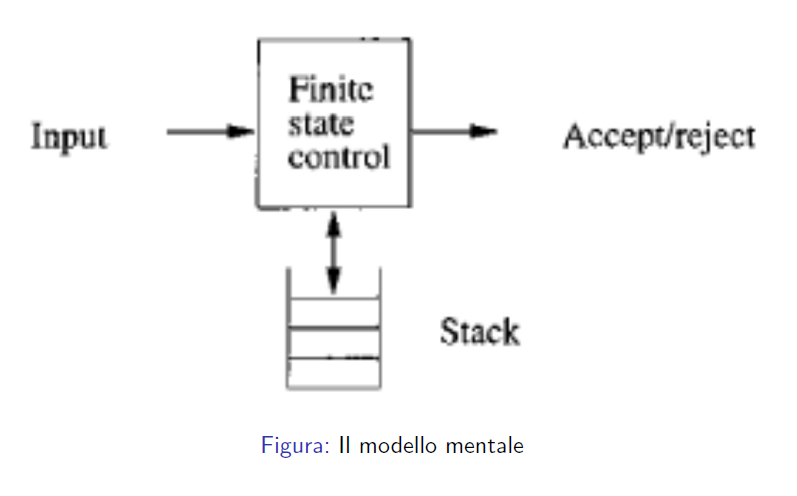
\includegraphics[width=6cm]{./Images/6.2.png}
\end{figure}
\FloatBarrier

\subsubsection{Definizione di automa a pila (Hopcroft, Motwani, Ullman)}
Definizione
Un automa a pila (o PDA) è una settupla
$\left(Q, \Sigma, \Gamma, \delta, q_{0}, Z_{0}, F\right)$
dove:
\begin{itemize}
    \item Q: Insieme finito degli stati
    \item $\Sigma$ : Alfabeto (finito) dei simboli input
    \item $\Gamma:$ Alfabeto (finito) dei simboli della pila
    \item $\delta: Q \times \Sigma_{\epsilon} \times \Gamma \rightarrow \mathcal{P}$ : funzione transizione, dove $\Sigma_{\epsilon}=\Sigma \cup\{\epsilon\}$ e $\mathcal{P}$ è un insieme finito di sottoinsiemi finiti di $Q \times \Gamma^{*}$.
    \item  $q_{0} \in Q:$ stato iniziale
    \item $Z_{0} \in \Gamma:$ simbolo iniziale
(la pila del PDA consiste all'inizio di una sola copia di questo simbolo)
    \item $F \subseteq Q:$ insieme degli stati finali
\end{itemize}
Quindi la funzione di transizione $\delta$ riceve come argomento una tripla $(q, a, X)$, dove $q$ è uno stato, a è un simbolo di input in $\Sigma$ oppure $a=\epsilon, X$ è un simbolo della pila, cioè un elemento $\mathrm{di} \Gamma$.

\vspace{5mm}

L'output di $\delta$, cioè $\delta(q, a, X)$, è un insieme finito di coppie $(p, \gamma)$, dove $p$ è il nuovo stato e $\gamma$ è la stringa di simboli di stack che rimpiazza $X$ alla sommità dello stack.

Ad esempio, se $\gamma=\epsilon$, il simbolo in cima alla pila viene eliminato; se $\gamma=X$, il simbolo in cima alla pila rimane invariato; se $\gamma=Y Z$, il simbolo in cima alla pila $X$ viene sostituito da $Z$ e $Y$ viene inserito nello stack.

\subsubsection{Definizione di Automa a pila (Sipser)}
Un automa a pila (o PDA) è una sestupla
$\left(Q, \Sigma, \Gamma, \delta, q_{0}, F\right)$ dove $Q, \Sigma, \Gamma$ ed $F$ sono tutti insiemi finiti, e
\begin{itemize}
    \item  Q è l'insieme degli stati,
    \item $\Sigma$ è l'alfabeto dell'input,
    \item $\Gamma$ è l'alfabeto della pila,
    \item $\delta: Q \times \Sigma_{\epsilon} \times \Gamma_{\epsilon} \rightarrow \mathcal{P}\left(Q \times \Gamma_{\epsilon}\right)$ è la funzione di transizione, dove $\Sigma_{\epsilon}=\Sigma \cup\{\epsilon\}$ e $\Gamma_{\epsilon}=\Gamma \cup\{\epsilon\}$,
    \item $q_{0} \in Q$ è lo stato iniziale,
    \item $F \subseteq Q$ è l'insieme degli stati accettanti (o finali).
\end{itemize}
La funzione di transizione $\delta$ riceve come argomento una tripla $(q, a, X)$, dove $q$ è uno stato, $a$ è un simbolo di input in $\Sigma$ oppure $a=\epsilon, X$ è un simbolo della pila, cioè un elemento di $\Gamma$ oppure $X=\epsilon$.

\vspace{5mm}

L'output di $\delta$, cioè $\delta(q, a, X)$, è un insieme finito di coppie $(p, Y)$, dove $p$ è il nuovo stato e $Y$ è un simbolo di stack che rimpiazza $X$ alla sommità dello stack oppure $Y=\epsilon$.


Ognuno dei simboli $a, X$ e $Y$ può essere $\epsilon$. 
\begin{itemize}
    \item Se a è $\epsilon$, la macchina può effettuare questa transizione senza leggere alcun simbolo dall'input.
    \item Se $X$ è $\epsilon$, la macchina può realizzare questa transizione senza leggere ed eliminare alcun simbolo dalla pila.
    \item Se $Y$ è $\epsilon$, la macchina non scrive alcun simbolo sulla pila durante questa transizione.
\end{itemize}

\subsubsection{Definizione di Automa a pila (confronto)}
È possibile dimostrare che le due definizioni sono equivalenti.

Nella definizione di Sipser manca il simbolo di fondo pila. Quindi questa definizione non contiene alcun meccanismo esplicito per permettere al PDA di controllare se la pila è vuota.

Sipser sottolinea che il PDA è in grado di ottenere lo stesso effetto inserendo inizialmente un simbolo speciale $\$$ nella pila. Se il PDA vede $\$$ di nuovo, sa che la pila è di fatto vuota.
Quindi, quando in una descrizione informale di un PDA si fa riferimento al controllo se la pila è vuota, per Sipser viene implicitamente implementata questa stessa procedura.

\begin{itemize}
    \item $\delta: Q \times \Sigma_{\epsilon} \times \Gamma \rightarrow \mathcal{P}$ funzione di transizione in Hopcroft, Motwani, Ullman;
    \item $\delta^{\prime}: Q \times \Sigma_{\epsilon} \times \Gamma_{\epsilon} \rightarrow \mathcal{P}\left(Q \times \Gamma_{\epsilon}\right)$ funzione di transizione in Sipser.
\end{itemize}

Sia $\left(p, Y_{1} \cdots Y_{n}\right) \in \delta(q, a, X), n \geq 1$. La transizione $\left(p, Y_{1} \ldots Y_{n}\right)$ viene simulata mediante $n$ applicazioni della $\delta^{\prime}$ (con stati intermedi supplementari). Ad esempio, se $(p, Y Z) \in \delta(q, a, X)$, la transizione $(p, Y Z)$ viene simulata mediante due applicazioni della $\delta^{\prime}$ (con stati intermedi supplementari).


Sia $(p, Y) \in \delta^{\prime}(q, a, \epsilon)$. La transizione $(p, Y)$ corrisponde alle transizioni $\delta(q, a, X)=(p, Y X)$, per ogni $X \in \Gamma$.

\subsubsection{Notazione grafica per i PDA}
Possiamo anche usare un diagramma di stato per descrivere un
PDA.

Tali diagrammi sono simili ai diagrammi di stato usati per
descrivere gli automi finiti, modificati per mostrare come il PDA
usa la sua pila quando passa da uno stato a un altro.

\subsubsection{Notazione grafica per i PDA (Hopcroft, Motwani, Ullman)}
Un PDA può essere descritto da un diagramma di transizione (o di stato).
E un grafo in cui:
\begin{itemize}
    \item I nodi corrispondono agli stati del PDA
    \item Lo stato iniziale ha una freccia entrante che non parte da alcun nodo (etichettata Start). Gli stati finali corrispondono ai nodi con un doppio cerchio.
    \item Vi è un arco dallo stato $q$ allo stato $p$ con etichetta $a, X / \alpha$ se $(p, \alpha) \in \delta(q, a, X)$.
\end{itemize}

\subsubsection{Notazione grafica per i PDA (Sipser)}
Nei diagrammi di stato di Sipser, le etichette hanno la forma $a, b \rightarrow c$.

Supponiamo che $a, b, c$ siano diversi da $\epsilon .$ Scriviamo " $a, b \rightarrow c$ " per indicare che, quando la macchina sta leggendo una a dall'input, essa può sostituire il simbolo $b$ sulla sommità della pila con una $c$.

Ognuno dei simboli $a, b$ e $c$ può essere $\epsilon$.
\begin{itemize}
    \item Se $a$ è $\epsilon$, la macchina può effettuare questa transizione senza leggere alcun simbolo dall'input.
    \item Se $b$ è $\epsilon$, la macchina può realizzare questa transizione senza leggere ed eliminare alcun simbolo dalla pila.
    \item Se $c$ è $\epsilon$, la macchina non scrive alcun simbolo sulla pila durante questa transizione.
\end{itemize}

\subsubsection{Esempio: Un PDA $P$ per $L=\left\{w w^{R} \mid w \in\{0,1\}^{*}\right\}$}

\begin{figure}[hbpt!]
    \centering
    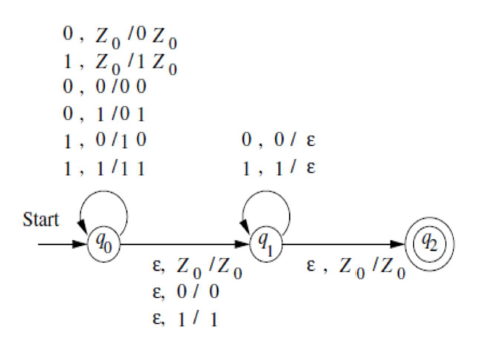
\includegraphics[width=8cm]{./Images/6.3.png}
\end{figure}
\FloatBarrier

\subsubsection{Esempio:
le parole palindrome di lunghezza pari su \{0; 1\}}

II PDA P per il linguaggio
$$
L=\left\{w w^{R} \mid w \in\{0,1\}^{*}\right\}
$$
può essere descritto da
$$
P=\left(\left\{q_{0}, q_{1}, q_{2}\right\},\{0,1\},\left\{0,1, Z_{0}\right\}, \delta, q_{0}, Z_{0},\left\{q_{2}\right\}\right)
$$
dove $\delta$ è definita dalle regole seguenti
\begin{enumerate}
    \item $\delta\left(q_{0}, 0, Z_{0}\right)=\left\{\left(q_{0}, 0 Z_{0}\right)\right\}, \quad \delta\left(q_{0}, 1, Z_{0}\right)=\left\{\left(q_{0}, 1 Z_{0}\right)\right\}$
    \item $\delta\left(q_{0}, 0,0\right)=\left\{\left(q_{0}, 00\right)\right\}, \quad \delta\left(q_{0}, 0,1\right)=\left\{\left(q_{0}, 01\right)\right\}$,
$\delta\left(q_{0}, 1,0\right)=\left\{\left(q_{0}, 10\right)\right\}, \delta\left(q_{0}, 1,1\right)=\left\{\left(q_{0}, 11\right)\right\}$
    \item $\delta\left(q_{0}, \epsilon, Z_{0}\right)=\left\{\left(q_{1}, Z_{0}\right)\right\}, \quad \delta\left(q_{0}, \epsilon, 0\right)=\left\{\left(q_{1}, 0\right)\right\}$,
$\delta\left(q_{0}, \epsilon, 1\right)=\left\{\left(q_{1}, 1\right)\right\}$
    \item $\delta\left(q_{1}, 0,0\right)=\left\{\left(q_{1}, \epsilon\right)\right\}, \quad \delta\left(q_{1}, 1,1\right)=\left\{\left(q_{1}, \epsilon\right)\right\}$
    \item $\delta\left(q_{1}, \epsilon, Z_{0}\right)=\left\{\left(q_{2}, Z_{0}\right)\right\}$
\end{enumerate}

\subsubsection{Esempio: Un PDA per le parole palindrome di lunghezza
pari su \{0, 1\}}

\begin{figure}[hbpt!]
    \centering
    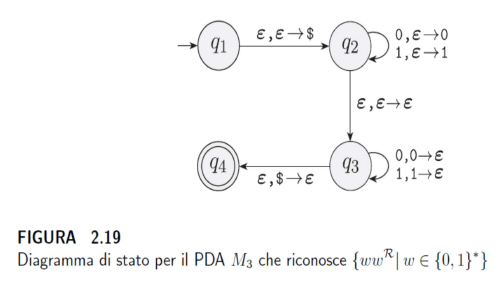
\includegraphics[width=8cm]{./Images/6.4.png}
\end{figure}
\FloatBarrier

\subsubsection{Esempio: Un PDA per $\left\{0^{n} 1^{n} \mid n \in \mathbb{N}, n \geq 0\right\}$}

\begin{figure}[hbpt!]
    \centering
    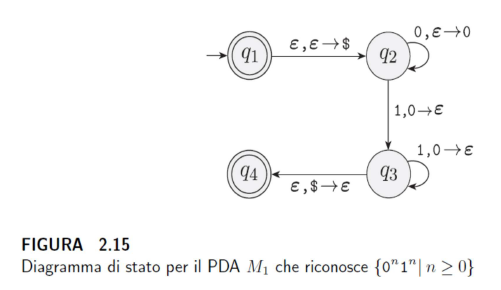
\includegraphics[width=8cm]{./Images/6.5.png}
\end{figure}
\FloatBarrier

\subsubsection{Esempio: Un PDA per $\left\{a^{i} b^{j} c^{k} \mid i, j, k \geq 0 e i=j\right.$ oppure $\left.i=k\right\}$}

\begin{figure}[hbpt!]
    \centering
    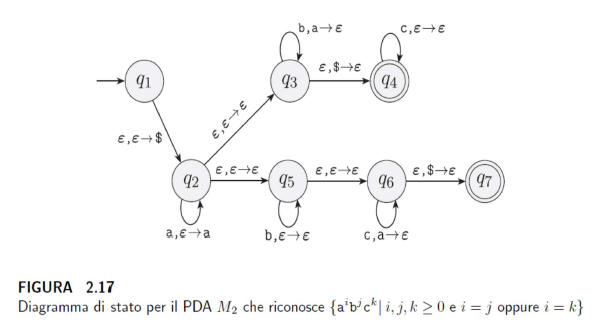
\includegraphics[width=9cm]{./Images/6.6.png}
\end{figure}
\FloatBarrier

\subsubsection{Descrizioni istantanee di un PDA}
Sia $P=\left(Q, \Sigma, \Gamma, \delta, q_{0}, Z_{0}, F\right)$ un PDA. Una descrizione istantanea (ID) (o configurazione) di un PDA è una tripla $(q, w, \gamma)$ dove
\begin{enumerate}
    \item $q$ è lo stato (corrente)
    \item $w$ è l'input residuo
    \item $\gamma$ è il contenuto della pila (convenzione: sommità della pila all'estremo sinistro di $\gamma$, quindi "alto $\rightarrow$ basso" corrisponde a "sinistra $\rightarrow$ destra").
\end{enumerate}

\subsubsection{Computazioni di un PDA}

Sia $P=\left(Q, \Sigma, \Gamma, \delta, q_{0}, Z_{0}, F\right)$ un PDA. Definiamo $\vdash_{P}$ ovvero $\vdash$ quando $P$ è sottointeso.
$\operatorname{Se}(p, \alpha) \in \delta(q, a, X)$ allora
$$
\forall w \in \Sigma^{*}, \beta \in \Gamma^{*} \quad(q, a w, X \beta) \vdash(p, w, \alpha \beta)
$$

\textbf{Nota:} $a w=w$ se $a=\epsilon$. Nota l'uso improprio del simbolo a sia per un carattere vero e proprio, che per la stringa vuota $\epsilon$ che non deve assolutamente essere considerata un carattere in lettura.

In un passo di calcolo dunque, l'automa o legge un carattere dall'input oppure non ne legge alcuno; rimuove un simbolo dalla pila; cambia stato; impila una stringa (anche vuota) di simboli.

\subsubsection{Computazioni di un PDA}

Definiamo $\underset{P}{\vdash}^{*}$ ovvero $\stackrel{*}{\vdash}$ quando $P$ è sottointeso.

\textbf{BASE}  $I \vdash^{*} /$ per qualunque ID $I .$

\textbf{INDUZIONE} $I \vdash^{*} J$ se esiste una ID $K$ tale che $I \vdash K$ e $K \vdash^{*} J$.

\subsubsection{Definizione ricorsiva delle stringhe di parentesi bilanciate}
\textbf{PASSO BASE:} La stringa vuota $\epsilon$ è una stringa di parentesi bilanciata.

\textbf{PASSO RICORSIVO: }Se $x$ e $y$ sono stringhe di parentesi bilanciate, allora anche $(x) y$ è una stringa di parentesi bilanciata.
$G_{\text {bal }}=(\{B\},\{(,)\}, P, B$, dove $P$ consiste nelle produzioni $B \rightarrow B B|(B)| \epsilon$
genera tutte e sole le stringhe di parentesi bilanciate.


\begin{figure}[hbpt!]
    \centering
    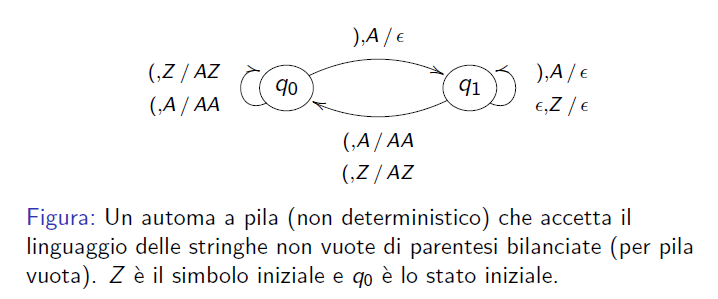
\includegraphics[width=9cm]{./Images/6.7.png}
\end{figure}
\FloatBarrier

$\begin{aligned}\left(q_{0},(()()), Z\right) &\left.\left.\left.\vdash\left(q_{0},()()\right), A Z\right) \vdash\left(q_{0},\right)()\right), A A Z\right) \\ &\left.\left.\left.\vdash\left(q_{1},()\right), A Z\right) \vdash\left(q_{0},\right)\right), A A Z\right) \\ &\left.\vdash\left(q_{1},\right), A Z\right) \vdash\left(q_{1}, \epsilon, Z\right) \vdash\left(q_{1}, \epsilon, \epsilon\right) \end{aligned}$

\begin{figure}[hbpt!]
    \centering
    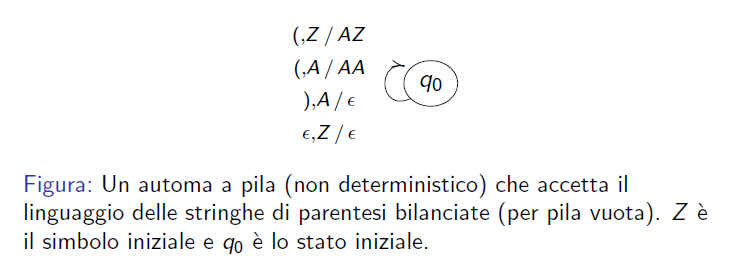
\includegraphics[width=9cm]{./Images/6.8.png}
\end{figure}
\FloatBarrier

$\begin{aligned}\left(q_{0},()(), Z\right) &\left.\vdash\left(q_{0},\right)(), A Z\right) \vdash\left(q_{0},(), Z\right) \\ &\left.\vdash\left(q_{0},\right), A Z\right) \vdash\left(q_{0}, \epsilon, Z\right) \\ & \vdash\left(q_{0}, \epsilon, \epsilon\right) \end{aligned}$

\subsubsection{Esempio:
le parole palindrome di lunghezza pari su \{a,b\}}

\begin{figure}[hbpt!]
    \centering
    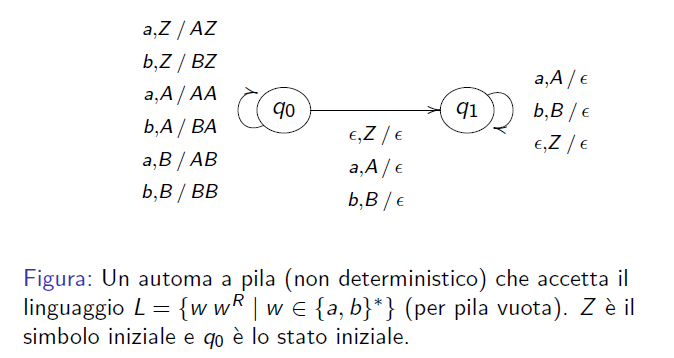
\includegraphics[width=9cm]{./Images/6.9.png}
\end{figure}
\FloatBarrier

$L=L(G), \operatorname{con} G=(\{S\},\{a, b\}, P, S)$ e

$P=\{S \rightarrow \epsilon|a S a| b S b\}$

\subsubsection{Esempio:
le parole palindrome di lunghezza pari su \{0,1\}}

\begin{figure}[hbpt!]
    \centering
    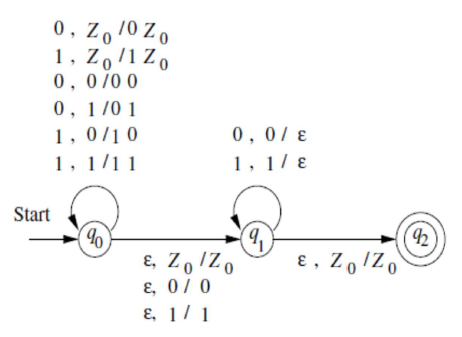
\includegraphics[width=9cm]{./Images/6.10.png}
\end{figure}
\FloatBarrier

\subsubsection{I linguaggi di un PDA}

\textbf{Definizione.} Sia $P=\left(Q, \Sigma, \Gamma, \delta, q_{0}, Z_{0}, F\right)$ un PDA. II linguaggio $L(P)$ accettato da $P$ per stato finale è
$$
L(P)=\left\{w \in \Sigma^{*} \mid \exists q \in F, \alpha \in \Gamma^{*} \text { tali che }\left(q_{0}, w, Z_{0}\right) \vdash_{P}^{*}(q, \epsilon, \alpha)\right\}
$$

\textbf{Nota.} Per definizione,
$$
\left(q_{0}, \epsilon, Z_{0}\right) \vdash_{P}^{*}\left(q_{0}, \epsilon, Z_{0}\right)
$$

Quindi se $q_{0} \in F$ allora $\epsilon \in L(P)$.

\subsubsection{Esempio:
le parole palindrome di lunghezza pari su \{0,1\}}


Siano $w \in\{0,1\}^{*}, x=w w^{R}$ e $P$ il PDA precedentemente definito.
La seguente computazione mostra che $x \in L(P)$.
$$
\begin{aligned}
&\left(q_{0}, w w^{R}, Z_{0}\right) \vdash^{*}\left(q_{0}, w^{R}, w^{R} Z_{0}\right) \vdash\left(q_{1}, w^{R}, w^{R} Z_{0}\right) \vdash^{*} \\
&\left(q_{1}, \epsilon, Z_{0}\right) \vdash\left(q_{2}, \epsilon, Z_{0}\right)
\end{aligned}
$$
\textbf{Nota}    La precedente relazione mostra che
$$
\left\{w w^{R} \mid w \in\{0,1\}^{*}\right\} \subseteq L(P) .
$$
È più difficile mostrare che
$$
L(P) \subseteq\left\{w w^{R} \mid w \in\{0,1\}^{*}\right\} .
$$

\subsubsection{I linguaggi di un PDA}

Sia $P=\left(Q, \Sigma, \Gamma, \delta, q_{0}, Z_{0}, F\right)$ un PDA. Definiamo $N(P)=\left\{w \in \Sigma^{*} \mid \exists q \in Q\right.$ tale che $\left.\left(q_{0}, w, Z_{0}\right) \vdash^{*}_P(q, \epsilon, \epsilon)\right\}$

Quindi $N(P)$ è l'insieme degli input $w$ che $P$ può consumare, svuotando nel contempo la pila.

Se interessa solo $N(P)$, l'insieme degli stati finali è in questo caso irrilevante e a volte $P$ viene scritto come una sestupla $\left(Q, \Sigma, \Gamma, \delta, q_{0}, Z_{0}\right)$.

Le due modalità di accettazione non modificano la classe dei linguaggi accettati.

\subsubsection{Da stack vuoto a stato finale}
\textbf{Teorema}

Se $L=N\left(P_{N}\right)$ per un PDA $P_{N}=\left(Q, \Sigma, \Gamma, \delta, q_{0}, Z_{0}\right)$, allora esiste un PDA $P_{F}$ tale che $L=L\left(P_{F}\right)$.

\begin{figure}[hbpt!]
    \centering
    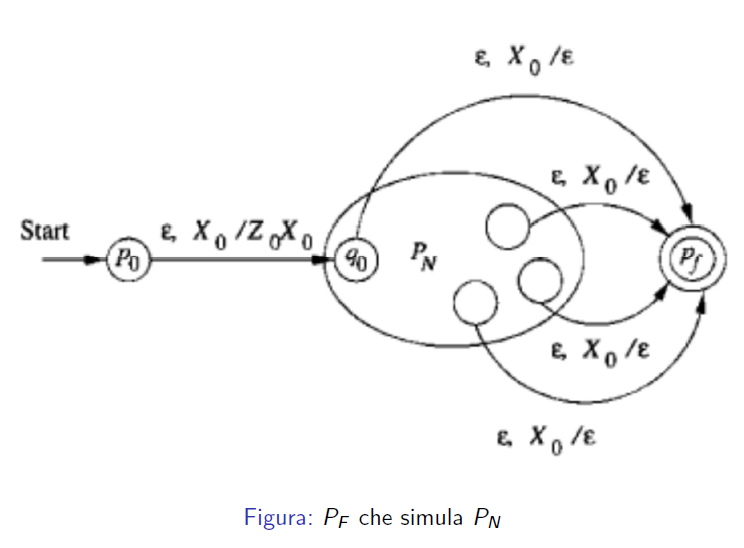
\includegraphics[width=9cm]{./Images/6.11.png}
\end{figure}
\FloatBarrier

\subsubsection{Esempio: le sequenze (scorrette) di \textit{if} ed \textit{else}}

\begin{figure}[hbpt!]
    \centering
    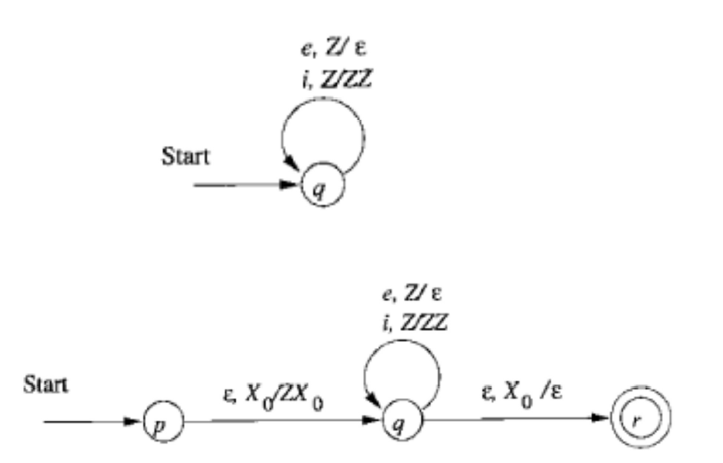
\includegraphics[width=9cm]{./Images/6.12.png}
\end{figure}
\FloatBarrier

\subsubsection{Da stato finale a stack vuoto}

\textbf{Teorema}

Sia $L=L\left(P_{F}\right)$ per un PDA $P_{F}=\left(Q, \Sigma, \Gamma, \delta, q_{0}, Z_{0}, F\right)$. Allora esiste un PDA $P_{N}$ tale che $L=N\left(P_{N}\right)$.

\begin{figure}[hbpt!]
    \centering
    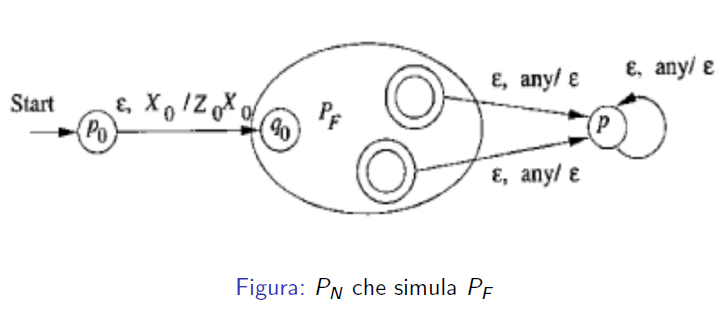
\includegraphics[width=9cm]{./Images/6.13.png}
\end{figure}
\FloatBarrier

\subsubsection{Computazione in un PDA (Sipser)}
\textbf{Definizione}

(Sipser) Un automa a pila $M=\left(Q, \Sigma, \Gamma, \delta, q_{0}, F\right)$ accetta un input
$w \quad$ se $w=w_{1} w_{2} \cdots w_{m}$, dove ciascun $w_{i} \in \Sigma_{\epsilon}$ ed esistono
$r_{0}, r_{1}, \ldots, r_{m} \in Q e s_{0}, s_{1}, \ldots, s_{m} \in \Gamma^{*}$ tali che
\begin{enumerate}
    \item $r_{0}=q_{0}$ and $s_{0}=\epsilon$. ( $M$ inizia nello stato iniziale e con una pila
vuota.)
    \item Per $i=0, \ldots, m-1,\left(r_{i+1}, b\right) \in \delta\left(r_{i}, w_{i+1}, a\right)$, dove $s_{i}=a t$ ed
$s_{i+1}=b t$ per qualche $a, b \in \Gamma_{\epsilon} e t \in \Gamma^{*} .(M)$ si muove
$\quad$ correttamente in base allo stato, al simbolo di pila, e al prossimo
simbolo in input.)
    \item  $r_{m} \in F$. (Alla fine dell'input $M$ si trova in uno stato accettante.)
\end{enumerate}
\textbf{Nota.} Come nella definizione di Hopcroft, Motwani, Ullman,
se $q_{0} \in F$ allora $\epsilon$ è accettata da M. Basta prendere $m=0$
nella precedente definizione.

\section{Automi a pila - Equivalenza CFG}

\subsubsection{Teorema - Da una grammatica CF a un PDA}

Data una grammatica context-free $G$ esiste un PDA P tale che $L(G)=N(P)$.

\vspace{5mm}

Data una grammatica context-free $G$ esiste un PDA P tale che $L(G)=L(P)$.

\subsubsection{Teorema - Da un PDA a una grammatica CF}
Dato un automa pushdown $P$ esiste una grammatica context-free $G$ tale che $L(G)=N(P)$.

\vspace{5mm}

Le grammatiche context-free e automi a pila definiscono la stessa
classe di linguaggi.
Si può dimostrare che per ogni CFG G esiste un PDA che
riconosce L(G) e per ogni PDA P esiste una CFG che genera L(P).
Le prove sono costruttive.

\subsubsection{Forma normale di Greibach}

Una grammatica context-free $G=(V, \Sigma, P, S)$ è in forma normale di Greibach se ogni sua produzione ha la forma
$$
A \rightarrow a \alpha, \quad \text { con } a \in \Sigma, \alpha \in V^{*} \text {. }
$$
Inoltre, se $S \rightarrow \epsilon \in P$, allora $S$ non compare alla destra di nessuna produzione.

Se $G$ è in forma normale di Greibach, ogni forma sentenziale in una derivazione a sinistra consiste in una stringa di terminali $x$ seguita da una stringa di variabili $\alpha$.

Cioè, data una grammatica in forma normale di Greibach $G$ e $w \in L(G)$, ogni derivazione diretta nella derivazione a sinistra di $w$ in $G$ genera uno dei simboli di $w$.

\vspace{5mm}

La grammatica seguente è in forma normale di Greibach e genera il linguaggio $\left\{a^{n} b^{n} \mid n \geq 1\right\}$.
$$
S \rightarrow a B \mid a S B \quad B \rightarrow b
$$

\subsubsection{Teorema}
Per ogni grammatica context-free $G$ esiste una grammatica $G^{\prime}$ tale che $L\left(G^{\prime}\right)=L(G)$ e $G^{\prime}$ è in forma normale di Greibach.

\textbf{Esempio.}

La grammatica con simbolo iniziale E e produzioni
$$
E \rightarrow(E+E)|a| b
$$
è equivalente alla grammatica in forma normale di Greibach con con simbolo iniziale $E$ e produzioni
$$
\begin{gathered}
E \rightarrow(E A E B|a| b, \\
A \rightarrow+, \quad B \rightarrow)
\end{gathered}
$$

\subsubsection{Da una grammatica CF a un PDA}
Data una grammatica in forma normale di Greibach $G$ e $w \in L(G)$, ogni derivazione diretta in una derivazione a sinistra di $w$ in $G$ genera uno dei simboli di $w$.

\textbf{Esempio 1.} Data $G^{\prime}$ definita da
$$
\begin{aligned}
E & \rightarrow(E A E B|a| b,\\
&A \rightarrow+, \quad B \rightarrow)
\end{aligned}
$$
la derivazione sinistra di $(a+(b+a))$ in $G^{\prime}$ è
$E \underset{l m}{\Rightarrow}(E A E B \underset{l m}{\Rightarrow}(a A E B  \underset{l m}{\Rightarrow}(a+E B \underset{l m}{\Rightarrow}(a+(E A E B B$
$\Rightarrow \quad(a+(b A E B B  \underset{l m}{\Rightarrow}(a+(b+E B B  \underset{l m}{\Rightarrow}(a+(b+a B B$
$\Rightarrow \quad \operatorname{lm}(a+(b+a) B  \underset{\operatorname{lm}}{\Rightarrow}(a+(b+a))$

\textbf{Esempio 2.} Data $G$ definita da
$$
S \rightarrow a B \mid a S B \quad B \rightarrow b
$$
la derivazione sinistra di $a a b b$ in $G$ è
$$
S \underset{\operatorname{lm}}{\Rightarrow} a S B \underset{\operatorname{lm}}{\Rightarrow} a a B B \underset{\operatorname{lm}}{\Rightarrow} a a b B \underset{\operatorname{lm}}{\Rightarrow} a a b b
$$

La derivazione di $w$ in $G$ diventa accettazione di $w$ (per pila vuota) nell'automa a pila $P$ equivalente.

$P$ simula la derivazione in $G$ memorizzando nella pila la stringa (in rosso) di variabili mentre consuma la stringa input (in blu).

Quindi per ogni simbolo $a^{\prime} \in\{a, b\}$ e variabile $X$ sul top della pila, l'automa può scegliere quale delle produzioni applicare tra quelle della forma $X \rightarrow a^{\prime} \alpha$ (nel caso generale potremmo avere $a^{\prime}=\epsilon$ )
Questo definisce la funzione $\delta$.

\vspace{5mm}

L'automa $P$ equivalente a $G$ avrà un solo stato $q$, alfabeto degli input $\{a, b\}$, alfabeto di pila $\{S, A, B\}$, simbolo di fondo pila $S$ e funzione di transizione definita come segue.
\begin{itemize}
    \item Le produzioni $S \rightarrow a B \mid$ aSB determinano $\delta(q, a, S)=\{(q, B),(q, S B)\}$
    \item  La produzione $B \rightarrow b$ determina $\delta(q, b, B)=\{(q, \epsilon)\}$
\end{itemize}
Ad esempio, alla derivazione
$$
S \underset{\operatorname{lm}}{\Rightarrow} a S B \underset{\operatorname{lm}}{\Rightarrow} a a B B \Rightarrow \underset{\operatorname{lm}}{a} a b B \underset{\operatorname{lm}}{\Rightarrow} a a b b
$$
corrisponde la computazione
$$
\begin{aligned}
(q, a a b b, S) & \vdash(q, a b b, S B) \vdash(q, b b, B B) \\
& \vdash(q, b, B) \vdash(q, \epsilon, \epsilon)
\end{aligned}
$$

\vspace{5mm}

\textbf{Esempio $1 .$}
Sia $G^{\prime}$ definita da
$$
E \rightarrow(E A E B|a| b, \quad A \rightarrow+, \quad B \rightarrow)
$$
L'automa $P^{\prime}$ equivalente a $G^{\prime}$ avrà un solo stato $q$, alfabeto degli input $\{a, b,+,(,)\}$ , alfabeto di pila \{E, A, B\}, simbolo di fondo pila $E$ e funzione di transizione definita come segue.
\begin{itemize}
    \item Le produzioni $E \rightarrow(E A E B|a| b$ determinano $\delta(q,(, E)=\{(q, E A E B)\}, \delta(q, a, E)=\{(q, \epsilon)\},$, $\delta(q, b, E)=\{(q, \epsilon)\} .$
    \item La produzione $A \rightarrow+$ determina $\delta(q,+, A)=\{(q, \epsilon)\}$
    \item La produzione $B \rightarrow)$ determina $\delta(q,), B)=\{(q, \epsilon)$,
\end{itemize}

Sia $G=(V, T, R, S)$ una CFG che, senza perdita di generalità, assumiamo sia in forma normale di Greibach. Possiamo anche supporre che $\epsilon \notin L(G)$, la costruzione va leggermente modificata per includere il caso in cui $\epsilon \in L(G)$.

Costruiamo allora l'automa a pila
$P=(\{q\}, T, V, \delta, q, S,\{q\})$, dove per ogni $a \in T$ e $A \in V$,

\begin{center}
    $(q, \gamma) \in \delta(q, a, A)$ se e solo se $A \rightarrow a \gamma$
\end{center}


Il PDA P simula una derivazione a sinistra di G. Poiché G è in forma normale di Greibach, ogni forma sentenziale in una derivazione a sinistra consiste in una stringa di terminali $x$ seguita da una stringa di variabili $\alpha$.
$P$ memorizza il suffisso $\alpha$ della forma sentenziale sinistra nella pila dopo aver letto il prefisso $x$.

\vspace{5mm}

Formalmente si può provare per induzione che
$$
S \underset{\operatorname{lm}}{\stackrel{*}{\Rightarrow}} x \alpha \text { se e solo se }(q, x, S) \stackrel{*}{\vdash}(q, \epsilon, \alpha)
$$
Questa relazione con $\alpha=\epsilon$ diventa
$$
S \underset{\operatorname{lm}}{\stackrel{*}{\Rightarrow}} x \text { se e solo se }(q, x, S) \stackrel{*}{\vdash}(q, \epsilon, \epsilon)
$$
Cioè $x$ è in $L(G)$ se e solo se $x \in N(P)$.

\vspace{5mm}

\textbf{Nota.} Attenzione al caso in cui $G$ è non ambigua!
\textbf{Nota.} Esercizio. Se $P$ è un PDA, esiste un PDA $P_{1}$ con un sol stato tale che $N\left(P_{1}\right)=N(P)$.

\vspace{5mm}

\textbf{Teorema}

Data una grammatica context-free G esiste un PDA P tale che
L(G) = L(P).

\subsubsection{Da un PDA a una grammatica CF}
Ora vogliamo dimostrare che, dato un PDA $P$, esiste una grammatica context-free $G$ tale che $N(P)=L(G)$. Inoltre, se $P$ è deterministico, allora $G$ è non ambigua.

La dimostrazione si basa sul prendere atto che l'evento cruciale nel processo di elaborazione di un input da parte di un PDA è l'eliminazione di un simbolo dalla pila in conseguenza della lettura di parte dell'input.

\vspace{5mm}

Nella figura seguente è raffigurata l'eliminazione di $Y_{j}$ dalla pila per effetto della lettura della stringa input $x_{j}$. Non avviene necessariamente in un sol passo, può richiedere più stati intermedi. Lo stato raggiunto alla fine è denotato in figura con $p_{j}$.

\begin{figure}[hbpt!]
    \centering
    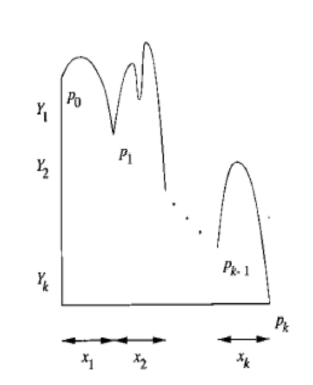
\includegraphics[width=6cm]{./Images/6.14.png}
\end{figure}
\FloatBarrier

Dato un PDA $P=\left(Q, \Sigma, \Gamma, \delta, q_{0}, Z_{0}\right)$ Le variabili della grammatica avranno la forma
$$
[p X q]
$$
con $p, q \in Q, X \in \Gamma$.
La variabile rappresenta un "evento" con due componenti:
\begin{itemize}
    \item l'eliminazione effettiva del simbolo $X$ dalla pila
    \item il passaggio dallo stato $p$ allo stato $q$, dopo la sostituzione di $X$ con $\epsilon$ sullo stack.
\end{itemize}

\textbf{Teorema}

Dato un automa pushdown $P=\left(Q, \Sigma, \Gamma, \delta, q_{0}, Z_{0}\right)$ esiste una grammatica context-free $G$ tale che $L(G)=N(P)$.

\vspace{5mm}

\textbf{Dimostrazione (Cenni)}

La grammatica richiesta è $G=(V, \Sigma, R, S)$, dove l'insieme delle variabili $V$ contiene
\begin{enumerate}
    \item il simbolo speciale $S$ come simbolo iniziale
    \item tutti i simboli $[p X q]$ con $p, q \in Q, X \in \Gamma$.
\end{enumerate}
Le produzioni in $G$ sono definite come segue:
\begin{enumerate}[(a)]
    \item Per ogni stato $p \in Q$,
$$
S \rightarrow\left[q_{0} Z_{0} p\right] \in R
$$
    \item Per ogni coppia $\left(r, Y_{1} Y_{2} \cdots Y_{k}\right) \in \delta(q, a, X)$, con $a \in \Sigma \cup\{\epsilon\}$, $k \geq 0$,
$$
\left[q X_{r_{k}}\right] \rightarrow a\left[r Y_{1} r_{1}\right]\left[r_{1} Y_{2} r_{2}\right] \cdots\left[r_{k-1} Y_{k} r_{k}\right] \in R
$$
per ogni sequenza di stati $r_{1}, \ldots r_{k} \in Q$.
\end{enumerate}

\subsubsection{Esempio: le sequenze scorrette di \textit{if} ed \textit{else}}

\begin{figure}[hbpt!]
    \centering
    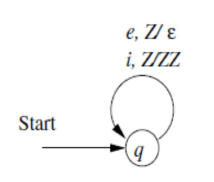
\includegraphics[width=5cm]{./Images/6.15.png}
\end{figure}
\FloatBarrier

\subsubsection{Esempio}

Sia $P_{N}=\left(\{q\},\{i, e\},\{Z\}, \delta_{N}, q, Z\right)$ con $\delta_{N}(q, i, Z)=\{(q, Z Z)\}, \quad \delta_{N}(q, e, Z)=\{(q, \epsilon)\}$
La grammatica $G=(V, \Sigma, P, S)$ tale che $L(G)=N\left(P_{N}\right)$ costruita nella prova è definita da
$$
\Sigma=\{i, e\}, \quad V=\{S,[q Z q]\}
$$
e produzioni:
$$
S \rightarrow[q Z q], \quad[q Z q] \rightarrow i[q Z q][q Z q], \quad[q Z q] \rightarrow e
$$
Ponendo $[q Z q]=A$, le produzioni diventano
$$
S \rightarrow A, \quad A \rightarrow i A A \mid e
$$
Una grammatica più semplice che genera lo stesso linguaggio:
$$
G^{\prime}=(\{S\},\{i, e\},\{S \rightarrow i S S \mid e\}, S)
$$

\subsubsection{Da un PDA a una grammatica CF}

\textbf{Teorema}

Dato un automa pushdown P esiste una grammatica context-free
G tale che L(G) = L(P).

\section{Proprietà di chiusura dei Linguaggi Context-Free}

I CFL sono chiusi rispetto all'unione, alla concatenazione e allo star di Kleene.
Ma non sono chiusi rispetto all'intersezione o alla differenza. E quindi non sono chiusi rispetto al complemento.

\subsubsection{Chiusura dei CFL rispetto all'
unione}

Siano L ed M due CFL con grammatiche
$\mathrm{G}$ e H, rispettivamente.

Assumiamo che G ed H non hanno
variabili in comune. I nomi delle variabili non influenzano il
linguaggio.

Siano S $_{1}$ ed S $_{2}$ i simboli iniziali di G e H.

\vspace{5mm}

Formiamo una nuova grammatica per $L \cup M$ prendendo tutti i simboli e le produzioni di Ge H.
Poi aggiungiamo un nuovo simbolo iniziale S.

Aggiungiamo le produzioni $\mathrm{S} \rightarrow \mathrm{S}_{1} \mid \mathrm{S}_{2}$.

\vspace{5mm}

Nella nuova grammatica, tutte le derivazioni iniziano con S.
Il primo passo sostituisce $\mathrm{S} \operatorname{con} \mathrm{S}_{1}$ o con $S_{2}$.

Nel primo caso, il risultato deve essere una stringa in $L(G)=L$ nel secondo caso una stringa in $\mathrm{L}(\mathrm{H})=\mathrm{M}$.

\subsubsection{Chiusura dei CFL rispetto alla
Concatenazione}

Siano L ed M due CFL con grammatiche $\mathrm{Ge} \mathrm{H}$, rispettivamente. Assumiamo che $\mathrm{G}$ ed $\mathrm{H}$ non hanno variabili in comune.

Siano $\mathrm{S}_{1}$ ed $\mathrm{S}_{2}$ i simboli iniziali di $\mathrm{Ge} \mathrm{H}$.

\vspace{5mm}

Formiamo una nuova grammatica per LM iniziando con tutti i simboli e le produzioni di $\mathrm{Ge} \mathrm{H}$.

Aggiungiamo un nuovo simbolo iniziale S.
Aggiungiamo la produzione $\mathrm{S} \rightarrow \mathrm{S}_{1} \mathrm{~S}_{2}$.

Ogni derivazione da S produce una
stringa in $\mathrm{L}$ seguita da una in $\mathrm{M}$.

\subsubsection{Chiusura rispetto allo Star}
Sia $L$ generato dalla grammatica $G$, con simbolo iniziale $S_{1}$.

Formiamo una nuova grammatica per $\mathrm{L}^{*}$ introducendo in $\mathrm{G}$ un nuovo simbolo iniziale S e le produzioni $\mathrm{S} \rightarrow \mathrm{S}_{1} \mathrm{~S} \mid \epsilon$.

Un derivazione (a destra) da S genera una sequenza di zero o più $\mathrm{S}_{1}$, ciascuno dei quali genera una stringa in $\mathrm{L}$.

\subsubsection{Chiusura dei CFL rispetto
all’inversione}

Se $L$ è un CFL con grammatica G, formiamo una grammatica per $L^{R}$ prendendo il "reverse" del lato destro di ogni produzione.

Esempio: Sia G definita da S -> OS1 | $01 .$ $\mathrm{L}(\mathrm{G})^{\mathrm{R}}$ è generato dalla grammatica S -> 1S0 | 10 .

\subsubsection{Non chiusura rispetto
all’Intersezione}

Diversamente dai linguaggi regolari, la
classe dei CFL non è chiusa rispetto a $\cap$.

Sappiamo che $L_{1}=\left\{0^{n} 1^{n} 2^{n} \mid n \geq 1\right\}$ non
Invece $L_{2}=\left\{0^{n} 1^{n} 2^{i} \mid n \geq 1, i \geq 1\right\}$ lo è.

CFG: $S \rightarrow A B, A \rightarrow 0 A 1|01, B \rightarrow 2 B| 2$.
$E$ lo è anche $L_{3}=\left\{0^{i} 1^{n} 2^{n} \| n \geq 1, i \geq 1\right\} .$
Ma $L_{1}=L_{2} \cap L_{3} .$

\subsubsection{Non chiusura rispetto alla
Differenza}

Possiamo provare qualcosa di più generale: ogni classe di linguaggi che è chiusa rispetto alla differenza è chiusa rispetto all'intersezione.

Prova: $L \cap M=L-(L-M)$.

Quindi, se i CFL fossero chiusi rispetto
alla differenza, sarebbero chiusi rispetto all'intersezione, ma non lo sono.

\subsubsection{Intersezione con un
linguaggio Regolare}

L'intersezione di due CFL non è necessariamente context free.
Ma l'intersezione di un CFL con un linguaggio regolare è sempre un CFL.

Prova: "eseguiamo" un DFA e un PDA in parallelo e notiamo che il risultato è un PDA: i PDA accettano per stato finale.

\subsubsection{DFA e PDA in Parallelo}

\begin{figure}[hbpt!]
    \centering
    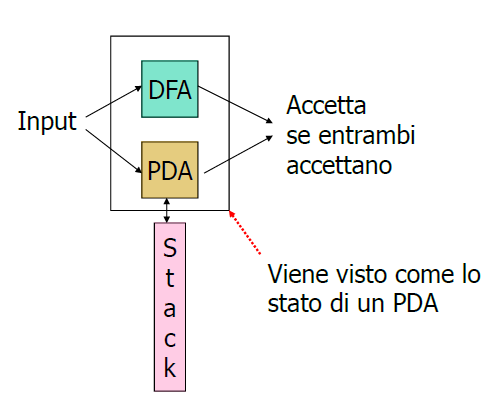
\includegraphics[width=7cm]{./Images/6.16.png}
\end{figure}
\FloatBarrier

\subsubsection{Costruzione formale}

\textbf{Nota:} In questa costruzione
useremo lo stesso simbolo per la
funzione di transizione e per la funzione
di transizione estesa del DFA A.

\vspace{5mm}

Sia $\delta_{A}$ la funzione di transizione del DFA A. Sia $\delta_{p}$ la funzione di transizione del PDA P. Gli stati del nuovo PDA sono $[q, p]$, dove $q$ è uno stato di A e p è uno stato di P. $\delta([q, p], a, X)$ contiene $\left(\left[\delta_{A}(q, a), r\right], \alpha\right)$ se $\delta_{p}(p, a, X)$ contiene $(r, \alpha)$.


Nota che a potrebbe essere $\varepsilon$, nel qual caso $\delta_{A}(q, a)=q .$

\vspace{5mm}

Gli stati finali del nuovo PDA sono gli stati $[q, p]$ tali che $q$ è uno stato finale di A e p è uno stato finale di P.

\vspace{5mm}

Facile induzione:

$\left(\left[q_{0}, p_{0}\right], w, z_{0}\right)\vdash^{*}([q, p], \varepsilon, \alpha)$
se e solo se
$\delta_{A}\left(q_{0}, w\right)=q$
e in $P:\left(p_{0}, w, Z_{0}\right)\vdash^{*}(p, \varepsilon, \alpha)$.

\section{Automi a pila deterministici}

\subsubsection{Definizione di Automa a pila deterministico (Hopcroft,
Motwani, Ullman)}

Un automa a pila deterministico (o DPDA) è un PDA $P=\left(Q, \Sigma, \Gamma, \delta, q_{0}, Z_{0}, F\right)$ che verifica le seguenti condizioni:
\begin{enumerate}
    \item Per ogni $q \in Q, a \in \Sigma_{\epsilon}, X \in \Gamma, \delta(q, a, X)$ ha al massimo un elemento.
    \item Se esiste $a \in \Sigma$ tale che $\delta(q, a, X) \neq \emptyset$ allora $\delta(q, \epsilon, X)=\emptyset$.
\end{enumerate}

\subsubsection{Linguaggi context-free deterministici}

Tutte le definizioni introdotte per un PDA (diagramma di stato, descrizione istantanea, computazione, linguaggio accettato per stati finali, linguaggio accettato per pila vuota) si applicano anche ai DPDA.

\vspace{5mm}


Un linguaggio L è un linguaggio context-free deterministico $(D C F L)$ se esiste un automa a pila deterministico $P$ tale che $L=L(P) .$


\subsubsection{\text { Un PDA non deterministico per }$\left\{w w^{R} \mid w \in\{0,1\}^{*}\right\}$}

\begin{figure}[hbpt!]
    \centering
    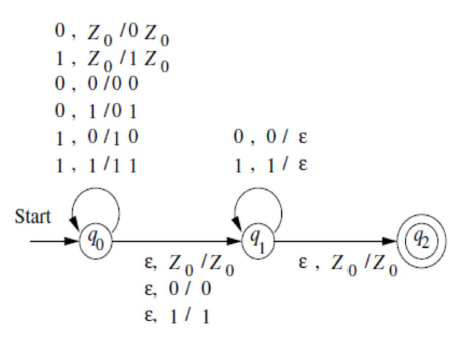
\includegraphics[width=7cm]{./Images/6.17.png}
\end{figure}
\FloatBarrier

$$
\left\{w C W^{R} \mid W \in\{0,1\}^{*}\right\} \text { è un } D C F L
$$
II linguaggio $\left\{w c w^{R} \mid w \in\{0,1\}^{*}\right\}$ è un linguaggio context-free deterministico.

\subsubsection{Esempio:
le stringhe di parentesi bilanciate}

\begin{figure}[hbpt!]
    \centering
    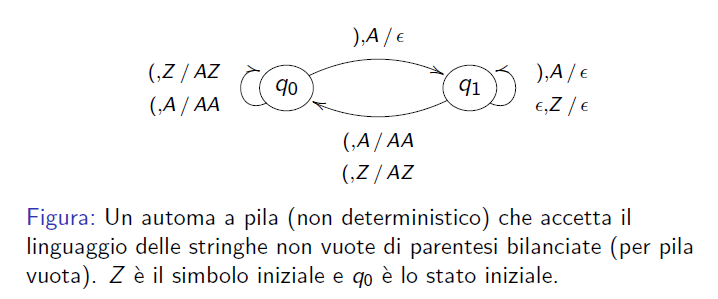
\includegraphics[width=7cm]{./Images/6.7.png}
\end{figure}
\FloatBarrier

II PDA non è un DPDA perché $\delta\left(q_{1}, \epsilon, Z\right) \neq \emptyset \mathrm{e}$ $\delta\left(q_{1},(, Z) \neq \emptyset\right.$.

\begin{figure}[hbpt!]
    \centering
    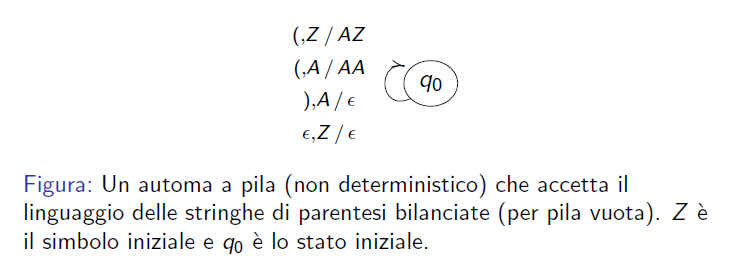
\includegraphics[width=7cm]{./Images/6.8.png}
\end{figure}
\FloatBarrier

II PDA non è un DPDA perché $\delta\left(q_{0}, \epsilon, Z\right) \neq \emptyset$ e $\delta\left(q_{0},(, Z) \neq \emptyset\right.$.

\subsubsection{Definizione di Automa a pila deterministico (Sipser)}
Un automa a pila deterministico (o DPDA) è una sestupla $\left(Q, \Sigma, \Gamma, \delta, q_{0}, F\right)$ dove $Q, \Sigma, \Gamma$ ed $F$ sono tutti insiemi finiti, e
\begin{itemize}
    \item Q è l'insieme degli stati,
    \item  $\Sigma$ è l'alfabeto dell'input,
    \item I è l'alfabeto della pila,
    \item $\delta: Q \times \Sigma_{\epsilon} \times \Gamma_{\epsilon} \rightarrow\left(Q \times \Gamma_{\epsilon}\right) \cup\{\emptyset\}$ è la funzione di transizione, dove $\Sigma_{\epsilon}=\Sigma \cup\{\epsilon\}$ e $\Gamma_{\epsilon}=\Gamma \cup\{\epsilon\}$,
    \item $q_{0} \in Q$ è lo stato iniziale,
    \item $F \subseteq Q$ è l'insieme degli stati accettanti (o finali).
    \item Per ogni $q \in Q, a \in \Sigma e x \in \Gamma$, esattamente uno dei valori
$$
\delta(q, a, x), \delta(q, a, \epsilon), \delta(q, \epsilon, x) \text { e } \delta(q, \epsilon, \epsilon)
$$
è diverso dal $\emptyset$.
\end{itemize}


\textbf{Nota:}

Se $\delta(q, a, x)=(r, y)$ allora M legge $a$, elimina $x$ dalla pila, passa nello stato $r$ ed inserisce $y$ sulla pila.

\vspace{5mm}

Invece, se $\delta(q, a, x)=\emptyset$ allora quando $M$ è nello stato $q$, non ha nessuna mossa per leggere a ed eliminare $x$. In questo caso, la condizione su $\delta$ richiede che uno tra $\delta(q, \epsilon, x), \delta(q, a, \epsilon), \circ \delta(q, \epsilon, \epsilon)$ sia diverso dal vuoto, e allora $M$ si muove di conseguenza.

È possibile dimostrare che la definizione di automa a pila
deterministico di Sipser e la definizione di automa a pila
deterministico di Ullman sono equivalenti.

\subsubsection{Linguaggi context-free e DPDA}

\textbf{Teorema}
Ogni linguaggio accettato da un DPDA (per stato finale o per pila vuota) è context-free.

Questo teorema si dimostra facilmente poiché, come nel caso degli automi finiti, un DPDA è un particolare PDA in cui per ogni transizione vi è una sola scelta possibile.
Ma non vale il viceversa. La versione non deterministica e quella deterministica di un PDA non sono equivalenti. Gli automi a pila non deterministici sono più potenti della loro controparte deterministica.

\vspace{5mm}

linguaggi che sono riconosciuti da automi a pila deterministici
(per stati finali) sono chiamati linguaggi context-free deterministici
(DCFL). Questa sottoclasse dei linguaggi context-free è importante
per le applicazioni, come il progetto di parser nei compilatori per i
linguaggi di programmazione, perché il problema del parsing è
generalmente più facile per i DCFL che per i CFL.

\vspace{5mm}

Il linguaggio
$$
L_{w w r}=\left\{w w^{R} \mid w \in\{0,1\}^{*}\right\}
$$
è un linguaggio context-free che non può essere riconosciuto da un DPDA per stati finali né per pila vuota.

\vspace{5mm}

\textbf{Proposizione}

La classe dei linguaggi context-free include strettamente la classe dei linguaggi riconosciuti da un DPDA. Quindi la classe dei linguaggi context-free include strettamente la classe dei linguaggi context-free deterministici.

\begin{figure}[hbpt!]
    \centering
    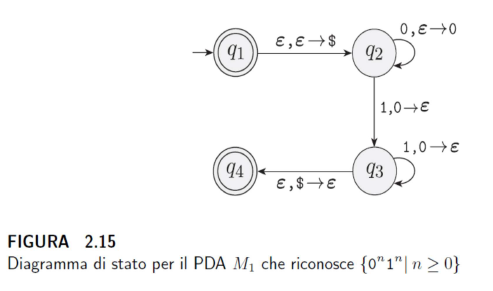
\includegraphics[width=9cm]{./Images/6.18.png}
\end{figure}
\FloatBarrier

\textbf{Esempio}

Il linguaggio $\left\{0^{n} 1^{n} \mid n \in \mathbb{N}, n \geq 0\right\}$ è un linguaggio context-free deterministico.

\vspace{5mm}

Possiamo facilmente trasformare il suo automa a pila $M_{1}$ in un automa a pila deterministico aggiungendo, per ogni combinazione di stato, simbolo di input e simbolo di pila mancante, transizioni a uno stato "trappola" da cui l'accettazione non è possibile.

\subsubsection{Esempio: Un PDA per $\left\{a^{i} b^{j} c^{k} \mid i, j, k \geq 0 e i=j\right.$ oppure $\left.i=k\right\}$}

\begin{figure}[hbpt!]
    \centering
    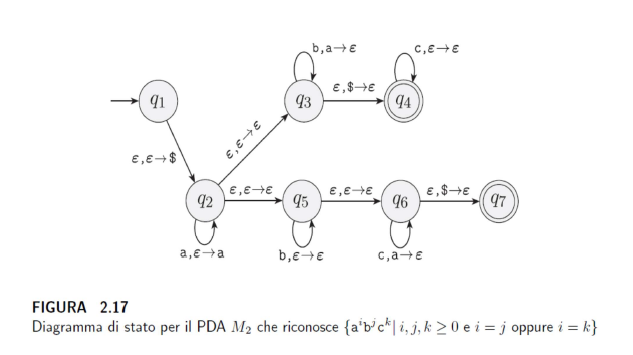
\includegraphics[width=9cm]{./Images/6.19.png}
\end{figure}
\FloatBarrier

\subsubsection{Linguaggi context-free e DPDA}

\textbf{Esempio}

I linguaggi context-free
$$
\begin{gathered}
L_{w w r}=\left\{w w^{R} \mid w \in\{0,1\}^{*}\right\} \\
\left\{a^{i} b^{j} c^{k} \mid i, j, k \geq 0 \text { e } i=j \text { oppure } i=k\right\}
\end{gathered}
$$
non sono linguaggi context-free deterministici: si può dimostrare che il non determinismo è necessario per riconoscere questi linguaggi.

\subsubsection{Proprietà di chiusura dei linguaggi context-free
deterministici}

La classe dei linguaggi context-free deterministici è chiusa rispetto al complemento.

Questo risultato si aggiunge alle proprietà di chiusura che un linguaggio context-free deterministico eredita dall'essere un linguaggio context-free. Precisamente,
\begin{itemize}
    \item se $L_{1}, L_{2}$ sono DCFL allora $L_{1} \cup L_{2}, L_{1} L_{2}, L_{1}^{*}$ sono $\mathrm{CFL}$,
    \item $\overline{L_{1}}$ è un DCFL.
\end{itemize}

La proposizione precedente fornisce un altro metodo per ottenere esempi di linguaggi context-free che non sono deterministici.
II linguaggio
$$
X=\left\{a^{i} b^{j} c^{k} \mid i \neq j \circ j \neq k, i, j, k \geq 0\right\}
$$
è un CFL ma non un DCFL, altrimenti
$$
X \cap L\left(a^{*} b^{*} c^{*}\right)=\left\{a^{n} b^{n} c^{n} \mid n \geq 0\right\}
$$
sarebbe context-free.

\vspace{5mm}

Il linguaggio
$$
X=\left\{a^{i} b^{j} c^{k} \mid i \neq j \circ j \neq k, i, j, k \geq 0\right\}
$$
è un $C F L$ ma non un $D C F L$.
Supponiamo per assurdo che $X$ sia un DCFL.
Allora anche $\bar{X}$ è un $D C F L$ e quindi $X$ è context-free.
Quindi
$$
X \cap L\left(a^{*} b^{*} c^{*}\right)=\left\{a^{n} b^{n} c^{n} \mid n \geq 0\right\}
$$
sarebbe context-free perché intersezione di un linguaggio context-free con uno regolare.

Ma utilizzando il pumping lemma, abbiamo visto che $\left\{a^{n} b^{n} c^{n} \mid n \geq 0\right\}$ non è context-free.

\vspace{5mm}

Il linguaggio
$$
X=\left\{a^{i} b^{j} c^{k} \mid i \neq j \circ j \neq k, i, j, k \geq 0\right\}
$$
è context-free perché è generato dalla grammatica definita dalle produzioni
$$
\begin{aligned}
&S \rightarrow A B \mid C D \\
&A \rightarrow a A \mid \epsilon \\
&B \rightarrow b B C|E| c D \\
&C \rightarrow a C b|E| a A \\
&D \rightarrow C D \mid \epsilon \\
&E \rightarrow b E \mid b
\end{aligned}
$$

\subsubsection{Proprietà di chiusura dei DCFL}

\begin{itemize}
    \item A genera zero o più $a, D$ genera zero o più $c, E$ genera zero o più $b$.
    \item B genera una stringa in $b^{*} c^{*}$ con un diverso numero di $b$ e $c$ (prima genera un ugual numero di $b$ e $c$, poi produce una o più $b$ (tramite $E$ ) oppure una o più $c$ (tramite $c D$ ).
    \item Analogamente C genera una stringa in $a^{*} b^{*}$ con un diverso numero di $a$ e $b$.
    \item Quindi $A B$ genera stringhe in $a^{*} b^{*} c^{*}$ con un diverso numero di $b$ e c mentre $C D$ genera stringhe in $a^{*} b^{*} c^{*}$ con un diverso numero di $a$ e $b$.
\end{itemize}

\subsubsection{Linguaggi regolari e DPDA}

\textbf{Teorema}

Se $L$ è un linguaggio regolare, allora esiste un DPDA P tale che $L=L(P)$. Quindi ogni linguaggio regolare è un linguaggio context-free deterministico.

\vspace{5mm}

\textbf{Prova (Cenni).}

Dato un DFA $\mathcal{A}$, esiste un DPDA $P$ tale che $L(\mathcal{A})=L(P) .$
II DPDA "ignora" la pila e simula $\mathcal{A}$.
Più formalmente, dato un DFA $\mathcal{A}=\left(Q, \Sigma, \delta_{\mathcal{A}}, q_{0}, F\right)$, definiamo $P=\left(Q, \Sigma,\left\{Z_{0}\right\}, \delta_{P}, q_{0}, Z_{0}, F\right)$, dove
$$
\delta_{P}\left(q, a, Z_{0}\right)=\left\{\left(p, Z_{0}\right)\right\}
$$
per ogni $p, q \in Q$ tali che $\delta_{\mathcal{A}}(q, a)=p$.
Si può dimostrare che
$$
\left(q_{0}, w, Z_{0}\right) \vdash^{*}_P\left(p, \epsilon, Z_{0}\right) \Leftrightarrow \hat{\delta_{\mathcal{A}}}\left(q_{0}, w\right)=p
$$
Poiché sia $\mathcal{A}$ che $P$ accettano entrando in uno degli stati di $F$, i loro linguaggi coincidono.


\vspace{5mm}

\textbf{Prova (Cenni).}
L'equivalenza
$$
\left(q_{0}, w, Z_{0}\right) \stackrel{*}{\digamma}_{P}\left(p, \epsilon, Z_{0}\right) \Leftrightarrow \delta_{\mathcal{A}}\left(q_{0}, w\right)=p
$$
è dimostrata mediante induzione su $|w|$.
II passo base è $|w|=0$, cioè $w=\epsilon$. In questo caso
$$
\begin{array}{lll}
\hat{\delta}_{\mathcal{A}}\left(q_{0}, \epsilon\right) & = & q_{0} \text { per definizione } \mathrm{di} \hat{\delta}_{\mathcal{A}} \\
\left(q_{0}, \epsilon, Z_{0}\right) & \stackrel{{ }}{P} & \left(q_{0}, \epsilon, Z_{0}\right) \text { per definizione di }
\end{array}
$$
Nella prova del passo induttivo occorre utilizzare il Teorema $6.5$ e il Teorema $6.6$ del testo di Hopcroft, Motwani, Ullman.

\subsubsection{Esempio}

Il linguaggio
$$
\left\{w c w^{R} \mid w \in\{a, b\}^{*}\right\}
$$
è un linguaggio context-free deterministico poiché è riconosciuto da un DPDA per stati finali (e per pila vuota).

\begin{figure}[hbpt!]
    \centering
    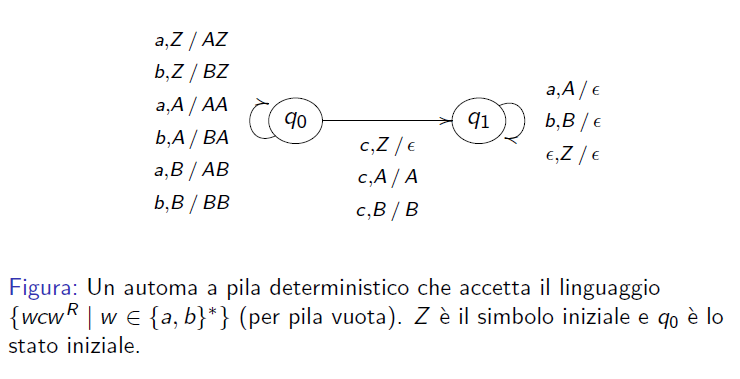
\includegraphics[width=8cm]{./Images/6.20.png}
\end{figure}
\FloatBarrier

\subsubsection{Linguaggi regolari e DPDA}

Il linguaggio
$$
L=\left\{w c w^{R} \mid w \in\{a, b\}^{*}\right\}
$$
non è regolare. Lo si dimostra applicando il pumping lemma alla stringa $a^{p}{ }_{C a}^{p}$.
Questo esempio e il teorema precedente ci permettono di concludere che la classe dei riconosciuti dai DPDA per stato finale (ovvero dei linguaggi context-free deterministici) include propriamente la classe dei linguaggi regolari.

\subsubsection{Linguaggi riconosciuti da DPDA}

Se consideriamo l'accettazione per pila vuota, la capacità di riconoscere linguaggi in questo modo è piuttosto limitata.

\textbf{Definizione}

Un linguaggio $L \subseteq \Sigma^{+}$è prefisso se $L \cap L \Sigma^{+}=\emptyset$.

Quindi in un linguaggio prefisso $L$ non esistono due stringhe diverse $x$ e $y$ tali che $x$ sia prefisso di $y$.

\vspace{5mm}

\textbf{Esempio.} Il linguaggio $\left\{w w^{R} \mid w \in\{0,1\}^{*}\right\}$ non è prefisso: la stringa 11 è prefisso di $1111 .$

\textbf{Esempio. }Il linguaggio $\{0\}^{*}$ non è prefisso: la parola vuota è prefisso di tutte le altre.

\textbf{Esempio.} Anche il linguaggio $\{0\}^{+}$non è prefisso. Infatti 0 è prefisso di 00 .

\textbf{Esempio. }Il linguaggio delle stringhe bilanciate non è prefisso: la stringa () è prefisso di ()() .

\vspace{5mm}

\textbf{Esempio.} II linguaggio $\left\{w c w^{R} \mid w \in\{a, b\}^{*}\right\}$ è prefisso. 

Supponiamo per assurdo che $x c x^{R}$ sia prefisso di $y c y^{R}$ e $x c x^{R} \neq y c y^{R} .$
Siccome tutte e due le stringhe hanno una sola occorrenza del carattere $c$, deve esistere $z \in\{a, b\}^{+}$tale che $y c y^{R}=x c x^{R} z$. Sempre utilizzando il fatto che abbiamo una sola occorrenza del carattere c dovremmo avere
$$
y=x, \quad y^{R}=x^{R} z
$$
Quindi
$$
|x|=|y|=\left|y^{R}\right|=\left|x^{R} z\right|>\left|x^{R}\right|=|x|
$$
il che è assurdo.

\vspace{5mm}

I linguaggi accettati dai DPDA per pila vuota sono tutti prefissi. Infatti sussiste il teorema seguente.

\vspace{5mm}

\textbf{Teorema}

Un linguaggio $L$ è $N(P)$ per un DPDA $P$ se e solo se $L$ è prefisso e $L=L\left(P^{\prime}\right)$ per un DPDA $P^{\prime}$.
\begin{itemize}
    \item  L'accettazione per stati finali e quella per pila vuota cessano di essere equivalenti nel caso deterministico.
    \item Non tutti i linguaggi regolari sono accettati da un DPDA per pila vuota.
Esempio: $\{0\}^{*}$.
\end{itemize}

\subsubsection{DPDA e grammatica CF non ambigue}

\textbf{Teorema}
Se $L=N(P)$ per un DPDA $P$, allora esiste una grammatica context-free non ambigua $G$ tale che $L(G)=N(P)$.

\vspace{5mm}

La prova consiste nel dimostrare che la costruzione della CFG equivalente a un PDA dato, quando è applicata a un DPDA P. fornisce una grammatica $G$ tale che ogni stringa generata da $G$ (quindi accettata dal $P$ ) ha un'unica derivazione a sinistra.

Sappiamo che questo è equivalente a dire che $G$ è non ambigua.

\vspace{5mm}

\textbf{Teorema}

Se $L=L(P)$ per un DPDA $P$, allora esiste una grammatica context-free non ambigua $G$ tale che $L(G)=L(P)$.


La prova di questo teorema è più laboriosa.

\subsubsection{Linguaggi marcati}

Dato un linguaggio $L$ su un alfabeto $\Sigma$, il linguaggio con simbolo di fine stringa (o linguaggio marcato) (associato ad L) è
$$
L \$=\{w \$ \mid w \in L\}
$$
$\operatorname{con} \$ \notin \sum .$
Notazione su Sipser: Il linguaggio marcato associato ad $L$ è denotato con $L \dashv$.

\subsubsection{Proprietà dei linguaggi marcati}

Per ogni linguaggio $L$ su un alfabeto $\Sigma$, il linguaggio marcato L\$ è un linguaggio prefisso.
Supponiamo per assurdo che $x \$$ sia prefisso di $y \$$, con $x, y \in L \subseteq \sum^{*} e x \$ \neq y \$$.
Siccome tutte e due le stringhe hanno una sola occorrenza del carattere $\$$, deve esistere $z \in \Sigma^{+}$tale che
$$
y \$=x \$ z
$$
Questo è impossibile.

\vspace{5mm}

Per ogni linguaggio $L$ su un alfabeto $\Sigma$, il linguaggio marcato $L \$$ è un linguaggio prefisso.


\textbf{Teorema}

Per ogni linguaggio $L$ su un alfabeto $\Sigma, L$ è il linguaggio accettato da un DPDA (per stati finali) se e solo se il corrispondente linguaggio marcato $L \$$ è il linguaggio accettato da un DPDA (per stati finali).

\vspace{5mm}

(Prova: vedi testo di Sipser)

\subsubsection{DPDA e grammatica CF non ambigue}

\textbf{Teorema}


Se $L=L(P)$ per un DPDA $P$, allora esiste una grammatica context-free non ambigua $G$ tale che $L(G)=L(P)$.
(Linee principali della prova.)
Sia $L=L(P)$ per un DPDA $P$.
Allora $L \$=L\left(P^{\prime}\right)$ per un DPDA $P^{\prime}$.
Quindi, essendo $L \$$ un DCFL prefisso, esiste un DPDA $P^{\prime \prime}$ tale che $L \$=N\left(P^{\prime \prime}\right)$ per un DPDA $P$.
Allora esiste una grammatica non ambigua $G^{\prime \prime}$ che genera $N\left(P^{\prime \prime}\right)=L \$ .$
Per ottenere da $G^{\prime \prime}$ una grammatica non ambigua $G$ che genera $L$ basta considerare $\$$ come una variabile di $G$ e aggiungere alle produzioni di $G^{\prime \prime}$ la produzione $\$ \rightarrow \epsilon$.

\vspace{5mm}

Invece non è sempre vero che un linguaggio non ambiguo è deterministico.

Esistono linguaggi $L$ tali che $L=L(G)$ con $G$ grammatica context-free non ambigua ma che non sono riconosciuti da alcun DPDA.
Un esempio è il linguaggio
$$
L_{w w r}=\left\{w w^{R} \mid w \in\{0,1\}^{*}\right\} .
$$
$L_{w w r}$ è un linguaggio che non può essere riconosciuto da un DPDA ma $L_{w w r}$ è generato dalla grammatica non ambigua $G=(\{S\},\{0,1\}, P, S)$, dove
$$
P=\{S \rightarrow \epsilon|0 S 0| 1 S 1\} .
$$

\subsubsection{Esempio:
le stringhe di parentesi bilanciate}

\begin{figure}[hbpt!]
    \centering
    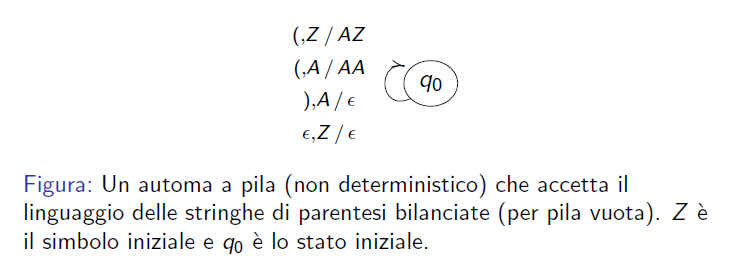
\includegraphics[width=7cm]{./Images/6.8.png}
\end{figure}
\FloatBarrier

$N(P)=\left\{w \$ \mid w \in\{(,)\}^{*}, w\right.$ è bilanciata $\}$

\subsubsection{DPDA e grammatiche deterministiche (Cenni)}

Esiste una nozione di grammatica context-free deterministica. Il modello è computazionalmente equivalente a quello degli automi a pila deterministici purché limitiamo la nostra attenzione ai linguaggi con simbolo di fine stringa.

Infatti si può provare che un linguaggio marcato è generato da una grammatica context-free deterministica se e solo se è un linguaggio context-free deterministico.

Non è una severa restrizione.

\vspace{5mm}

I linguaggi context-free deterministici sono di considerevole importanza per le applicazioni. I loro algoritmi per l'appartenenza e il parsing sono basati sui DPDA e (quindi) sono efficienti. Inoltre abbracciano un'ampia classe di CFL che include la maggior parte dei linguaggi di programmazione. Tuttavia, le grammatiche context-free deterministiche sono a volte scomode per esprimere particolari DCFL.

\vspace{5mm}

Per questa ragione nel parsing si considera una classe "più ampia" di grammatiche, chiamate grammatiche $L R(k)$, dove $k$ denota un intero non negativo.

Le grammatiche context-free deterministiche corrispondono alle grammatiche $L R(0)$.
È possibile mostrare che per ogni $k$ e per ogni grammatica $G$ che sia $L R(k)$, esiste un DPDA equivalente a $G$.
Poiché i DPDA sono equivalenti alle grammatiche $L R(0)$, le grammatiche $L R(k)$ sono tutte computazionalmente equivalenti per ogni $k$ e tutte descrivono esattamente i DCFL.







\let\cleardoublepage\clearpage

